\chapter{Лекция 3 — 24 февраля 2025}

\section{Представление атома в памяти}

Атом представлен в памяти пятью указателями. Последний из них -- package, был добавлен
на будущее развитие языка, первоначально представлял заглушку.

\begin{figure}[H]
    \begin{imagebox}
        \centering
        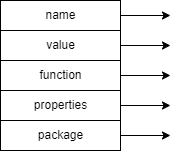
\includegraphics[height=0.2\textwidth]{img/atom.drawio.png}
        \label{fig:atom-in-memory}
    \end{imagebox}
    \caption{Представление атома в памяти}
\end{figure}

\section{set, setq}

SET требует ровно два аргумента. 
Значением первого аргумента должен быть атом, а значением 
второго - произвольное S-выражение. Функция присваивает атому, 
являющемуся значением первого аргумента, значение второго аргумента. 
Это значение возвращается в качестве результата. 

Функция SETQ отличается от SET тем, что не вычисляет значение 
первого аргумента. Поэтому первый аргумент при вызове SETQ не 
нужно квотировать. В остальном функция SETQ эквивалентна функции SET.

\begin{figure}[H]
    \begin{listingbox}{}
        \lstinputlisting[language=Lisp]{lists/set-setq.lisp}
    \end{listingbox}
    \caption{Пример работы функций set и setq}
    \label{lst:set-setq-example}
\end{figure}

\section{setf}

SETF — это макрос. Он позволяет делать присваивания в произвольное 
место. Первым аргументом SETF может быть как выражение, так и имя 
переменной. SETF позволяет устанавливать значение сразу нескольким
переменным.

\begin{figure}[H]
    \begin{listingbox}{}
        \lstinputlisting[language=Lisp]{lists/setf.lisp}
    \end{listingbox}
    \caption{Пример работы setf}
    \label{lst:setf-example}
\end{figure}

\section{cond, if}

В cond отбирается первое подвыражение, чья форма условия вычисляется 
в не-nil. Все остальные подвыражения игнорируются. Формы отобранного 
подвыражения последовательно выполняются.

В if выполняется форма test. Если результат не равен nil, 
тогда выбирается форма then. Иначе выбирается форма else. 
Выбранная ранее форма выполняется, и if возвращает то, что 
вернула это форма.

\begin{figure}[H]
    \begin{listingbox}{}
        \lstinputlisting[language=Lisp]{lists/if-cond.lisp}
    \end{listingbox}
    \caption{Пример работы if и cond}
    \label{lst:if-cond-example}
\end{figure}

\section{Логические операторы and, or, not}

NOT возвращает t, если аргумент является nil, иначе возвращает nil.
Функции NOT и null полностью эквиваленты. По соглашению принято 
использовать null, когда надо проверить пустой ли список, и NOT, 
когда надо инвертировать булево значение.

AND последовательно слева направо вычисляет формы. Если какая-либо 
форма formN вычислилась в nil, тогда немедленно возвращается 
значение nil без выполнения оставшихся форм. Если все формы кроме 
последней вычисляются в не-nil значение, AND возвращает то, что 
вернула последняя форма.

OR последовательно выполняет каждую форму слева направо. Если 
какая-либо непоследняя форма выполняется в что-либо отличное от nil, 
OR немедленно возвращает это не-nil значение без выполнения 
оставшихся форм. Если все формы кроме последней, вычисляются в nil, 
OR возвращает то, что вернула последняя форма. 

\begin{figure}[H]
    \begin{listingbox}{}
        \lstinputlisting[language=Lisp]{lists/and-or-not.lisp}
    \end{listingbox}
    \caption{Пример работы and, or, not}
    \label{lst:and-or-not-example}
\end{figure}

\section{let и let*}

LET используют, чтобы связать значение с символом таким образом, 
чтобы интерпретатор не спутал переменную с таким же именем, 
но определенную вне функции. 

Локальные переменные, создаваемые выражением LET, сохраняют свои 
значения только внутри самого выражения LET.

Символы в списке переменных -- это переменные, которым особая форма 
LET присваивает начальное значение. Если символ только один, то 
ему присваивается значение nil; если символ входит в состав 
двухэлементного списка, то ему назначается значение, которое 
возвращается после вычисления второго элемента списка.

Функция LET* отличается от LET только тем, что при вычислении 
значения очередной переменной из списка доступны значения уже ранее 
вычисленных переменных (последовательное вычисление).

\begin{figure}[H]
    \begin{listingbox}{}
        \lstinputlisting[language=Lisp]{lists/let.lisp}
    \end{listingbox}
    \caption{Пример работы let}
    \label{lst:let-example}
\end{figure}